\documentclass[]{ximera}
%handout:  for handout version with no solutions or instructor notes
%handout,instructornotes:  for instructor version with just problems and notes, no solutions
%noinstructornotes:  shows only problem and solutions

%% handout
%% space
%% newpage
%% numbers
%% nooutcomes

%I added the commands here so that I would't have to keep looking them up
%\newcommand{\RR}{\mathbb R}
%\renewcommand{\d}{\,d}
%\newcommand{\dd}[2][]{\frac{d #1}{d #2}}
%\renewcommand{\l}{\ell}
%\newcommand{\ddx}{\frac{d}{dx}}
%\everymath{\displaystyle}
%\newcommand{\dfn}{\textbf}
%\newcommand{\eval}[1]{\bigg[ #1 \bigg]}

%\begin{image}
%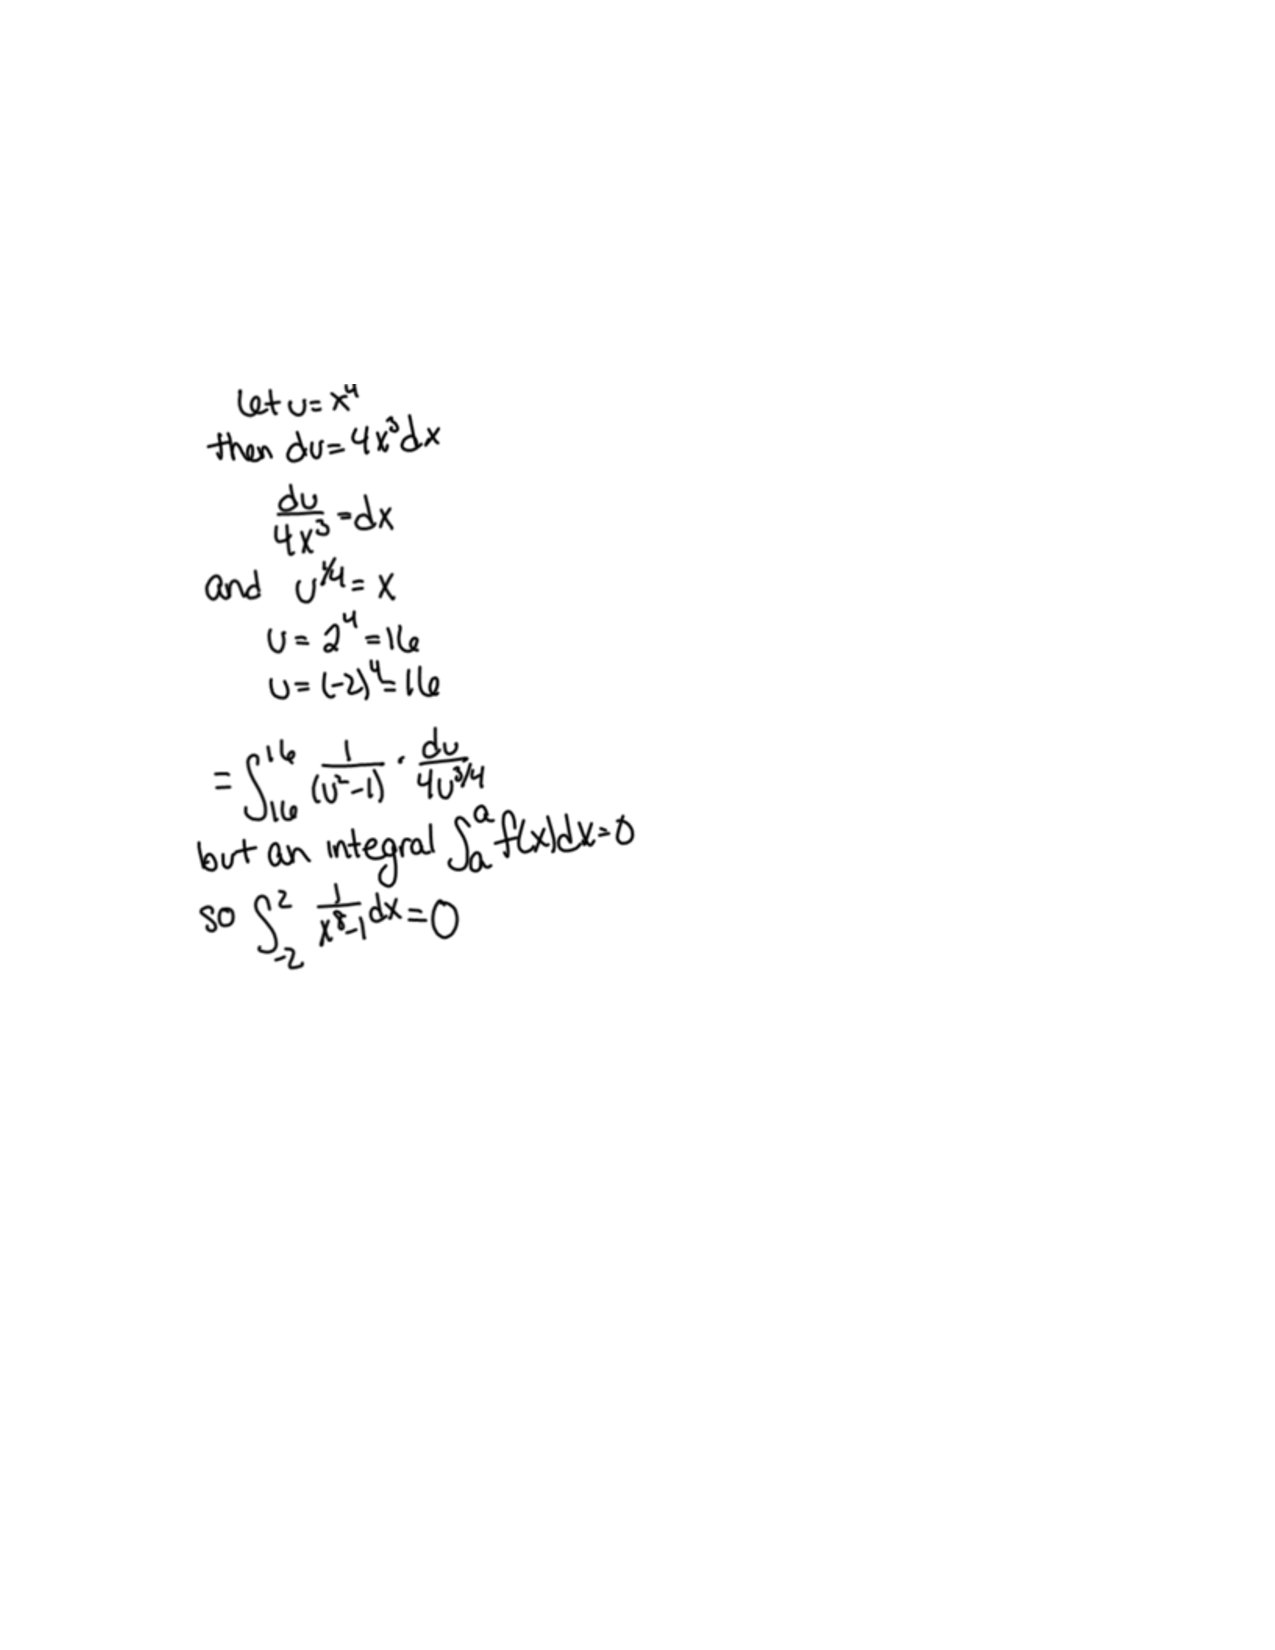
\includegraphics[trim= 170 420 250 180]{Figure1.pdf}
%\end{image}

%add a ``.'' below when used in a specific directory.
\newcommand{\RR}{\mathbb R}
\renewcommand{\d}{\,d}
\newcommand{\dd}[2][]{\frac{d #1}{d #2}}
\renewcommand{\l}{\ell}
\newcommand{\ddx}{\frac{d}{dx}}
\newcommand{\dfn}{\textbf}
\newcommand{\eval}[1]{\bigg[ #1 \bigg]}

\usepackage{multicol}

\renewenvironment{freeResponse}{
\ifhandout\setbox0\vbox\bgroup\else
\begin{trivlist}\item[\hskip \labelsep\bfseries Solution:\hspace{2ex}]
\fi}
{\ifhandout\egroup\else
\end{trivlist}
\fi} %% we can turn off input when making a master document

\title{Separable differential equations}  

\begin{document}
\begin{abstract}		\end{abstract}
\maketitle



\begin{comment}
\section{Warm up:}

	\begin{freeResponse}
	
	\end{freeResponse}
	
\begin{instructorNotes}

\end{instructorNotes}
\end{comment}







\section{Group work:}



%problem 1
\begin{problem}
Which of the following are separable differential equations?
For those that are, solve them, assuming that $y(4)=5$.
	\begin{enumerate}
	\item 	$y' = x^2+y^2$
	\begin{freeResponse}
	This differential equation is \dfn{not} separable.
	\end{freeResponse}
	
	
	
	\item 	$y'=x+xy^2$
	\begin{freeResponse}
		\begin{align*}
		&y' = x+xy^2  \\
		\Longrightarrow 	\qquad	&\dd[y]{x} = x(1+y^2)  \\
		\Longrightarrow 	\qquad	&\frac{\d y}{1+y^2} = x \d x.
		\end{align*}
	So this equation \dfn{is} separable.
	To solve, we integrate both sides of the equation:
		\begin{align}
		&\int \frac{1}{1+y^2} \d y = \int x \d x  \nonumber \\
		\Longrightarrow 	\qquad	&\arctan(y) = \frac{1}{2} x^2 + C  \label{equation 1 for y}\\
		\Longrightarrow 	\qquad	&y = \tan \left( \frac{1}{2} x^2 + C \right).  \nonumber
		\end{align}
	To find $C$, we plug the initial condition $y(4) = 5$ into equation \eqref{equation 1 for y} and solve for $C$.
		\begin{align*}
		&\arctan(5) = \frac{1}{2} (4)^2 + C = 8 + C  \\
		\Longrightarrow 	\qquad	&C = \arctan(5) - 8.
		\end{align*}
	So
		\[
		y = \tan \left( \frac{1}{2} x^2 + \arctan(5) - 8 \right).
		\]
	\end{freeResponse}
	
	
	
	\item 	$y' = e^{2x-y}$
	\begin{freeResponse}
		\begin{align}
		&y' = e^{2x-y}  \nonumber \\
		\Longrightarrow 	\qquad	&\dd[y]{x} = \frac{e^{2x}}{e^y}  \nonumber \\
		\Longrightarrow 	\qquad	&e^y \d y = e^{2x} \d x  \label{eqn 2}
		\end{align}
	and so this \dfn{is} a separable equation.  
	To solve, we integrate both sides of equation \eqref{eqn 2}.
		\begin{align}
		&\int e^y \d y = \int e^{2x} \d x  \nonumber  \\
		\Longrightarrow 	\qquad	&e^y = \frac{1}{2} e^{2x} + C  \label{eqn 3}  \\
		\Longrightarrow 	\qquad	&y = \ln \left( \frac{1}{2} e^{2x} + C \right).  \nonumber
		\end{align}
	To find $C$, we plug into equation \eqref{eqn 3} and solve for $C$:
		\begin{align*}
		&e^5 = \frac{1}{2} e^8 + C  \\
		\Longrightarrow 	\qquad	&C = e^5 - \frac{1}{2} e^8.
		\end{align*}
	Therefore
		\[
		y = \ln \left( \frac{1}{2} e^{2x} + e^5 - \frac{1}{2}e^8 \right).
		\]
	\end{freeResponse}
	\end{enumerate}
	
\end{problem}

\begin{instructorNotes}
Part (b) is the only non-separable equation.  
Students may need help recognizing that they can divide by the entire right side of both sides.  
Also, some results may only define $y$ implicitly.
\end{instructorNotes}







\begin{comment}
%problem 2
\begin{problem}

	\begin{freeResponse}
	
	\end{freeResponse}
		
\end{problem}

\begin{instructorNotes}

\end{instructorNotes}
\end{comment}







\begin{comment}
%problem 3
\begin{problem}

	\begin{freeResponse}
	
	\end{freeResponse}

\end{problem}

\begin{instructorNotes}

\end{instructorNotes}
\end{comment}
















	
	
	
	
	
	
	
	
	

	










								
				
				
	














\end{document} 


















